\section{3D Rekonstruktion}
\subsection{Tool Ökosystem}
Als zentrales Werkzeug zur Verarbeitung dreidimensionaler Informationen wurde die Pointcloud Library (PCL) \footnote{\url{http://www.poindclouds.org}} aufgrund von vorhandenen Vorkenntnissen des Autors identifiziert. PCL ist ein umfangreiches OpenSource C++ Framework zur Verarbeitung von Punktwolken. In mehreren Bibliotheksmodulen bietet PCL Implementierungen von gängigen Algorithmen zur Verarbeitung von räumlichen Information.\\
PCL selber verwendet ein Anzahl gängiger Bibliotheken zur Datenrepräsentation und -verarbeitung:

\begin{itemize}
		\item Boost 1.55 \footnote{\url{http://www.boost.org}} - für Shared Pointer
		\item Eigen3 \footnote{\url{http://http://eigen.tuxfamily.org}} - Matrizen, Vektoren, Lineare Algebra
		\item flann \footnote{\url{http://www.cs.ubc.ca/research/flann/}} - Fast Library for Approximate Nearest Neighbours
		\item QT \footnote{\url{http://qt-project.org/}}- GUI Framework
		\item vtk 6.1 \footnote{\url{http://www.vtk.org/}} - Visualization ToolKit
		\item qHull \footnote{\url{http://www.qhull.org/}} - Triangulation (COnvex/Concave Hull, Delaunay, Voronoi usw.)
		\item OpenNI2 \footnote{\url{http://structure.io/openni}} - zur Einbindung OpenNI-kompatibler Sensoren
		\item CUDA \footnote{\url{https://developer.nvidia.com/about-cuda}} - für GPU Implementierungen verschiedener Algorithmen
\end{itemize}

Diese Vielzahl von Abhängigkeiten sowie der Entwicklungszyklus von PCL haben einen großen Anteil am Aufwand zum Aufsetzen der Produktionsumgebung. Da vor allem die GPU-beschleunigten Verfahren sowie die Einbindung neuerer OpenNI2-kompatibler Sensoren noch nicht im neuesten Release eingebunden sind, ist die eigene Kompilierung der Bibliothek im aktuellen Stand der Entwicklung erforderlich. Im Laufe der Projekt 1 Veranstaltung wurde dies teilweise am tagesaktuellen Entwicklungsstand von PCL durchgeführt.\\

\subsection{Verwendete Module}
\begin{itemize}
	\item Common
	\item IO
	\item Filter
	\item Registration
	\item Surface
\end{itemize}

\subsection{Architektur}
Die Daten verschiedener Sensoren werden über ein gemeinsames Interface entgegengenommen. 
Die Verarbeitung der Sensordaten zu Polygonmeshes wird in einer Pipeline konfiguriert. Dafür werden verschiedene Punkt- und Meshprozessoren definiert, die in unterschiedlicher Weise kombiniert werden können. Punktprozessoren

\onecolumn

\begin{figure}[h!]
	\begin{center}		
		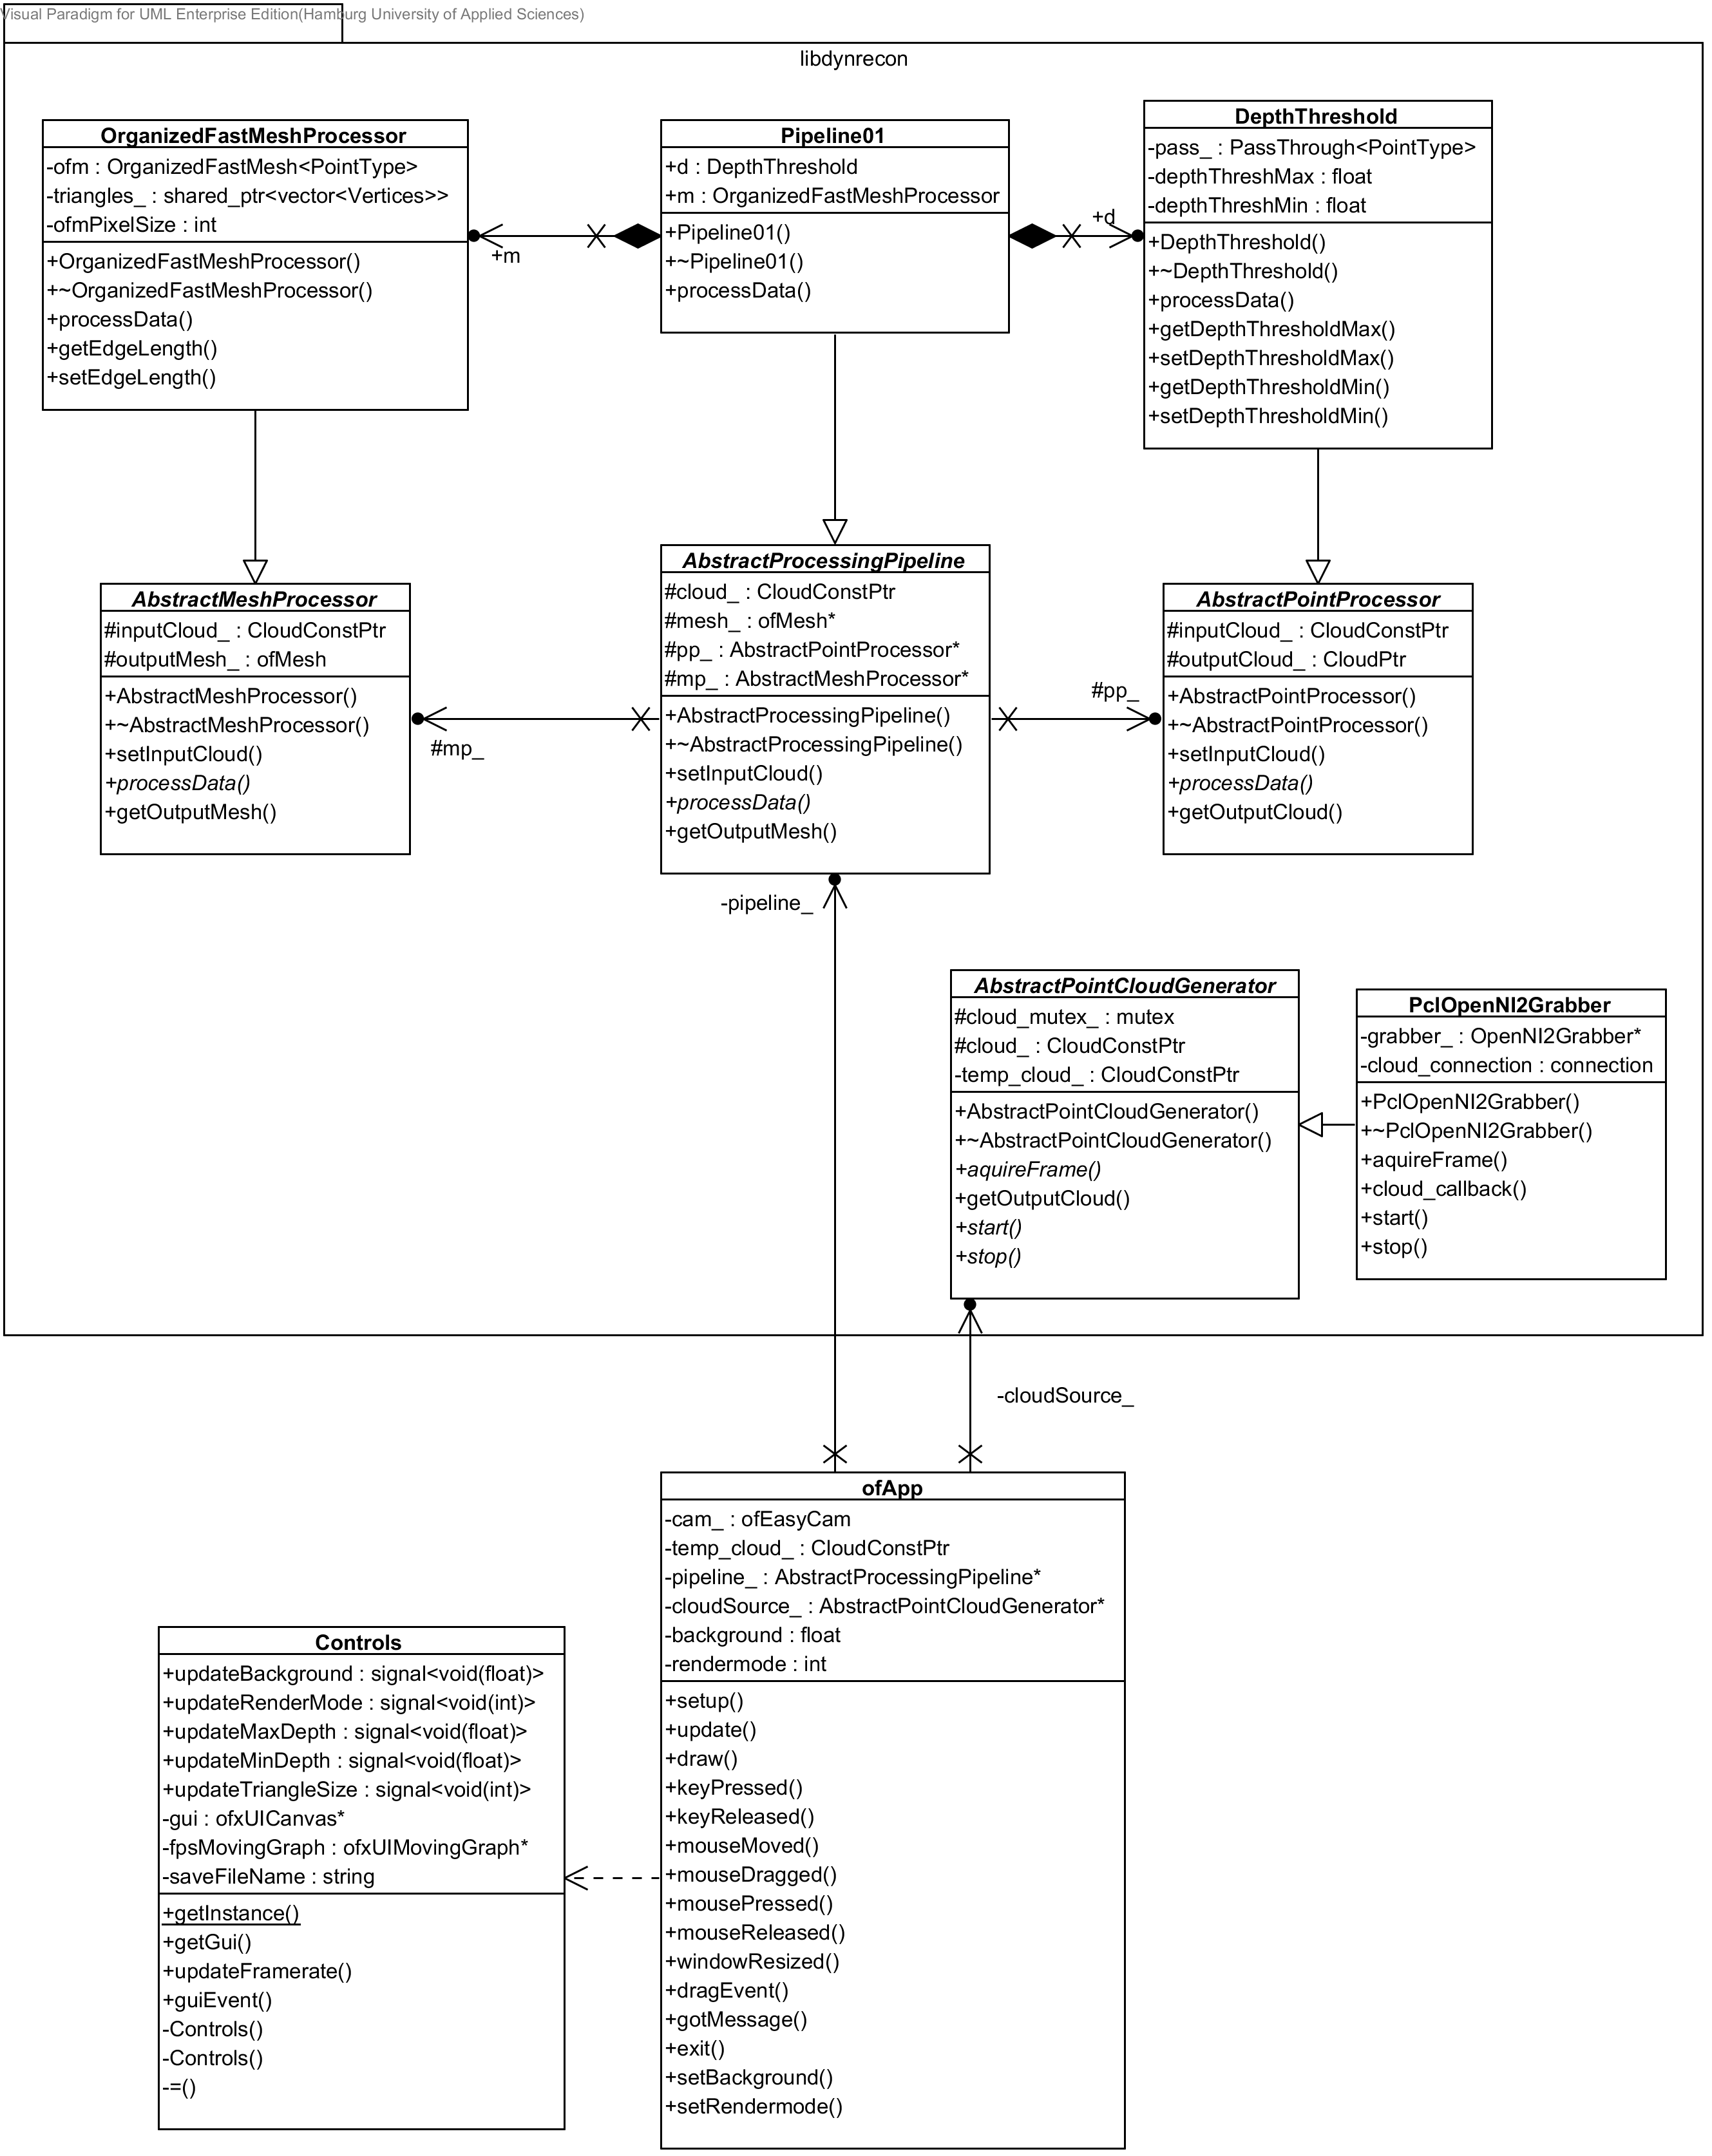
\includegraphics[width=.9\textwidth, keepaspectratio]{img/class_diagram}
		\caption{Klassen Diagramm}
	\end{center}
\end{figure}

\twocolumn

Blablabla
